\documentclass{article}
\usepackage{graphicx}
\usepackage[utf8]{inputenc}

\title{Opinions Dynamic Analisys}
\author{Biancone Saverio}
\date{Ottobre 2020}

\begin{document}

\maketitle

\section{Introduzione}
[ALLA FINE]
\section{La dinamica delle opinioni}
La dinamica delle opinioni ha come obiettivo quello di sviluppare dei modelli matematici volti a descrivere l'evoluzione delle opinioni all'interno di una rete sociale formata da individui interagenti.\\
\subsection{Lo studio}
Il sistema preso in esame, definito binario, prevede l'esistenza di due opinioni adottabili, che d'ora in poi indicheremo con opinione 0 e 1. Gli individui del sistema esprimeranno una preferenza verso una delle due opinioni, che definiremo  dominante\footnote{la definizione di opinione dominante dipende dal contesto ed esula dagli obiettivi di questo scritto}.\\
Senza perdità di generalità assumeremo 1 come tale.\\
Il sistema evolve in passi. Inizialmente ogni individuo condivide l'opinione 0.\\
Ad ogni passo, un individuo scelto casualmente adotta l'opinione 1 (dominante) con probabilità $\alpha$, mentre con probabilità 1-$\alpha$ adotta una delle due opinioni possibili attraverso delle dinamiche prestabilite.\\
Le dinamiche di aggiornamento dell'opinione prese in considerazione sono:
\begin{itemize}
\item Voter-Model, nel quale l'individuo adotterà l'opinione di uno dei suoi vicini scelto casualmente
\item Majority-Dynamic, nel quale l'individuo adotterà l'opinione più diffusa tra i suoi vicini
\end{itemize}
L'obiettivo è quello di analizzare il numero di passi, in valore atteso, necessari affinchè si raggiunga il consenso verso l'opinione dominante. È facile notare come, raggiunto questo stato, il sistema non possa evolvere più. Definiremo perciò tale stato "Stato di Assorbimento". \\
Tale analisi è volta a rivelare, qualora esistesse, il legame che intercorre tra la struttura della rete e il numero di passi necessari a raggiungere lo stato di assorbimento, sotto una specifica dinamica.

\subsection{Lo stato dell'arte}
[DA SVILUPPARE] 

\section{I test eseguiti}
 L'obbiettivo dietro lo sviluppo di questo software è stato quello di poter comparare ed analizzare statisticamente i tempi di assorbimento relativi a diverse topologie e modelli, tra cui:
 \begin{itemize}
\item Ipercubo
\item Clique
\item Ciclo
\item *Modello di Erdős–Rényi*
\end{itemize}
I primi test eseguiti sono serviti a verificare l'accuratezza del software e correggerne eventuali errori. Ogni test è composto da 100 simulazioni, configurate con Majority-Dynamic e bias pari a 0.5.\\
I test sono stati eseguiti su ipercubi, cliques e cicli, in dimensioni che vanno da $2^{5^{\mathrm{}}}$ fino a $2^{12^{\mathrm{}}}$ vertici.\\
\begin{center}
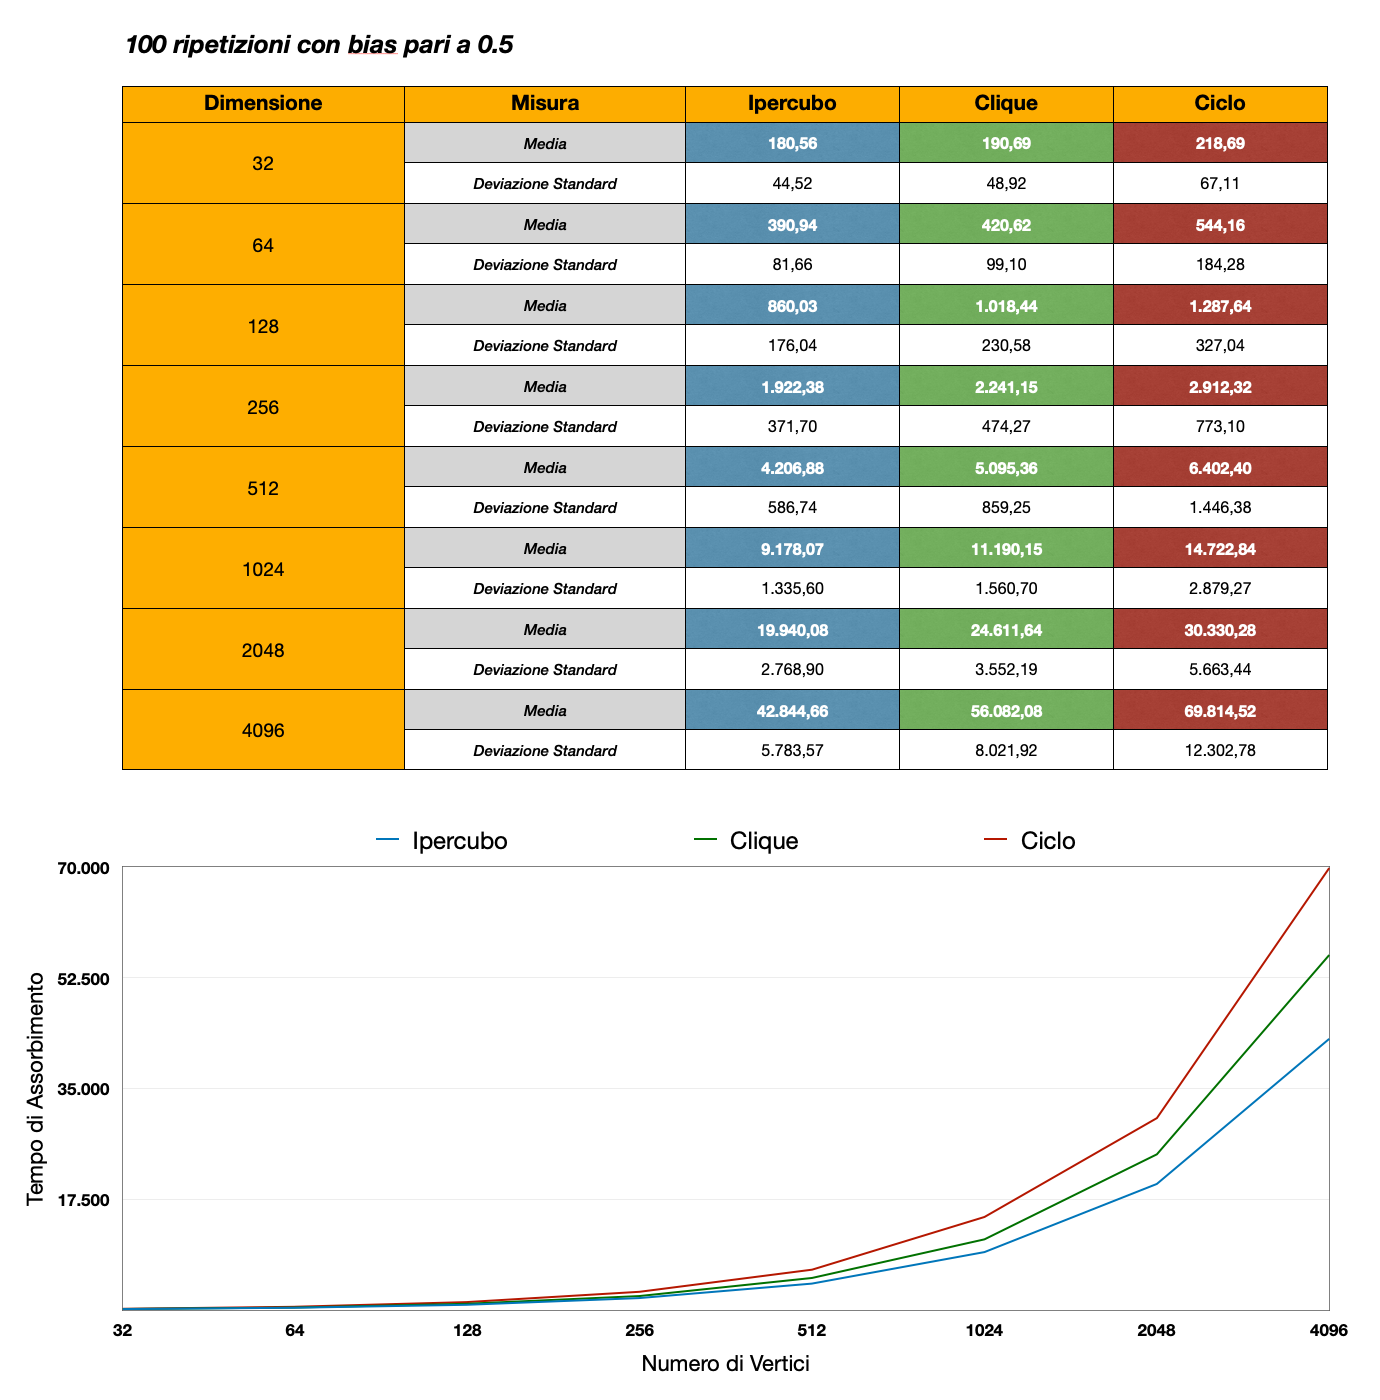
\includegraphics[width=1\textwidth]{test_bias05.png}
\end{center}
I risultati ottenuti sono perfettamente in linea con quanto dimostrato teoricamente. Per quanto riguarda il ciclo, dal [Th 4.4], il tempo di assorbimento è stato pari a $O(\frac{1}{\alpha}n\log{}n)$. \\
Per quanto riguarda clique e ipercubi, per i quali il grado minimo è pari a $\Omega(\log{}n)$, il tempo di assorbimento con bias pari a 0.5 si è rivelato essere $O(n\log{}n)$, anche questa volta confermando quanto evidenziato da [INSERIRE RIFERIMENTO].\\
Una volta appurato perciò che il software simulasse correttamente i processi descritti, ottenendo risultati conformi a quanto atteso, sono stati eseguiti test metodologicamente analoghi ai precedenti, adottando però un bias verso l'opinione dominante pari a 0.25, di fatto dimezzandolo.\\
\begin{center}
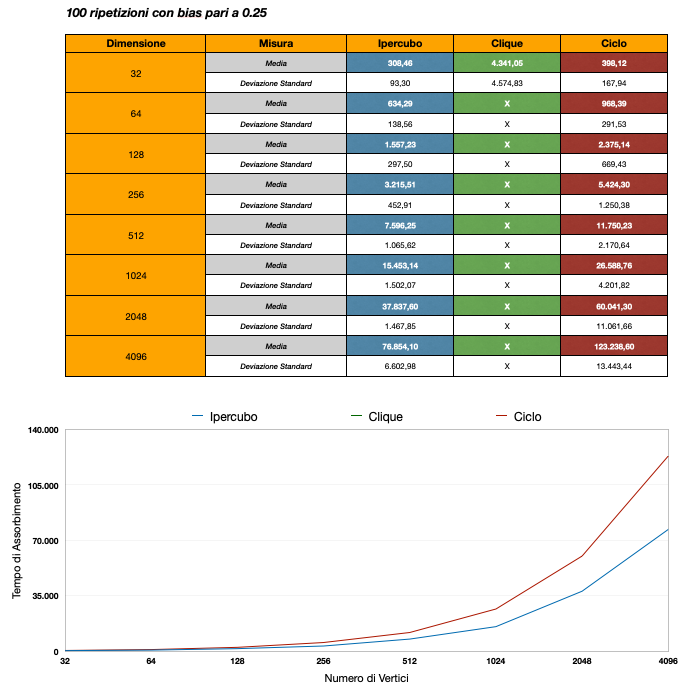
\includegraphics[width=1\textwidth]{test_bias025.png}
\end{center}
Per quanto riguarda il ciclo e la clique, sono stati ancora una volta confermati i risultati attesi.
Lo stato di assorbimento per il ciclo è stato nuovamente raggiunto in $O(\frac{1}{\alpha}n\log{}n)$ passi in valore atteso. Nello specifico, dimezzando il valore del bias, i tempi di assorbimento per tale topologia sono raddoppiati, suggerendo una proporzionalità inversa tra il numero di vertici e il valore del bias.\\
D'altra parte, come previsto, è stato impossibile ultimare i test per la clique, in quanto, con un bias inferiore a 0.5, il numero di passi necessari a raggiungere lo stato di assorbimento è diventato esponeziale nel numero di vertici, di fatto rendendo impossibile lo svolgimento dei test, già dalla dimensione di $2^{7^{\mathrm{}}}$.\\
Il paper [INSERIRE RIFERIMENTO], d'altronde, lascia aperta la domanda inerente al comportamento dell'ipercubo con un bias così basso. Dal risultato dei test si evince come l'ipercubo abbia un comportamento assimilabile a quello del ciclo, raggiungendo perciò lo stato di assorbimento in $O(n\log{}n)$ passi. 

\section{Opinion Dynamic Simulator}
Il software sviluppato ha lo scopo di fornire degli strumenti volti ad indagare statisticamente alcune delle dinamiche prese in esame, al fine di poter riprodurre tali dianimiche ed eventualmente fornire ulteriori risposte su topologie e meccaniche rimaste inesplorate.\\
Il linguaggio principale che è stato scelto per lo sviluppo del softaware è Python. Le motivazioni dietro tale scelta risiedono non soltanto nella grande diffusione e nel grande supporto di cui questo linguaggio gode, ma anche dalla preseza di numerosi moduli che permettessero al meglio di rappresentare ed interfacciarsi con i grafi, struttura attraverso la quale viene rappresentata la rete sociale.
Tra i vari moduli disponibili, è stato scelto Graph-Tool. Tra i punti di forza di questo modulo si annoverano una precisia modellazione di tali strutture, con possibilià di aggiungere proprietà personalizzate su vertici e archi e numerose funzioni di generazione e rappresentazione di alcune topologie tipiche dei grafi quali paths, cicli e cliques. Il vero punto di forza di Graph-Tool però è la sua velocità, ottenuta grazie alla possibilità di eseguire molte di queste funzioni, non in python, bensì in C, linguaggio di livello più basso e perciò più rapido nell'esecuzione di alcune istruzioni fondamentali.\\
Alcune topologie non presenti nativamente nel modulo, sono state personalmente riscritte utilizzando comunque le strutture di base fornite. É questo il caso dell'ipercubo, per il quale ho scritto un algoritmo di generazione basato sull'algoritmo Bit-Fix.\\
Partendo da tale base, è stato sviluppato il processo di simulazione vero e proprio. Tale processo necessita come input, oltre al grafo, di un configurator. L'oggetto configurator permette di fornire al simulatore le informazioni relative alle meccaniche con le quali si svolgerà la simulazione, come ad esempio la dinamica adottata e il bias verso l'opinione dominante.\\ 
Al termine del processo di simulazione, verranno salvate diverse informazioni quali:
\begin{itemize}
\item Un file .XML contenente la serializzazione del grafo.
\item Un file .XML contenente le informazioni di configurazione e il risultato (numero di step) della             simulazione.
\item Una rappresentazione grafica del grafo in formato .PNG
\item Una cartella contenente dei file .PNG che mostrano l'andamento evolutivo della simulazione.
\end{itemize}
La scelta del formato .XML è dettata dalla necessità di avere quante più informazioni possibili salvate in maniera strutturata. Inoltre python possiede nativamente un modulo per auto-formattare correttamente i file scritti in tale formato.
Le rappresentazioni grafiche invece sono state salvate in .PNG in quanto risultava essere un buon compromesso tra qualità dell'output e dimensione dei file stessi. Altre opzioni possibili sono .SVG e .PDF.\\

Al fine di ottenere dei dati quanto più possibile affidabili, e limitare l'aleatorietà di tali processi, il software dispone un modulo volto all'esecuzione di test. In questo contesto, per test si intende l'esecuzione ripetuta di una simulazione, mantenendo invariati i paramentri di configurazione e la struttura del grafo. Cosi come le simulaizoni anche i test necessitano di una configurazione, che include, oltre al numero di iterazioni da effettuare, l'oggetto configurator che verrà condiviso dalle simulazioni.\\
Al termine del test, verranno salvate diverse informazioni quali:
\begin{itemize}
\item Un file .XML contenente la serializzazione del grafo.
\item Un file .XML contenente le informazioni di configurazione del test, i risultati di ogni singola             simulazione, la media di tali risultati e la devizione standard
\item Una rappresentazione grafica del grafo in formato .PNG (OPZIONALE)
\end{itemize}
Ponendo come obiettivo quello di velocizzare l'esecuzione di un test e ridurre l'impatto in termini di dimensioni, soprattutto per grafi molto numerosi e/o densi, l'esecuzione di un test non comporta il savataggio di tutte le informazioni relative alle singole simulazioni.\\
Considerando la durata media di un test composto da 100 simulazioni eseguito su un grafo particolarmente  impegnativo come una Clique di $2^{12^{\mathrm{}}}$ vertici, ho scelto di inserire un modulo che permettesse di riunificare molteplici test pre-eseguiti, utilizzando come dataset l'insieme delle simulazioni eseguite e ricalcolando correttamente la media e la deviazione standard. \\
In questo modo è possibile suddividere un test composto da 100 simulazioni in 10 test indipendenti, da 10 simulazioni ognuno, permettendo cosi di ridurre sensibilmente lo stress computazionale inflitto alla macchina sul quale viene eseguito.


\end{document}
